\chapter{Proposta de tese}

\section{Problemas}\label{problemas}

Embora a modelagem geológica implícita com funções distância assinaladas seja uma metodologia bem estabelecida que permite ao gemodelador gerar de forma rápida modelos geológicos reprodutíveis, consistentes e checáveis a partir de uma função volume derivada a partir dos dados amostrais, existem alguns pontos problemáticos e limitantes na metodologia que merecem atenção.

A não estacionariedade da função distância assinalada torna a modelagem dos variogramas arbitrária e questionável.

Apesar dos métodos implícitos serem totalmente independentes de um \textit{grid}, o objetivo final da modelagem geológica implícita é preencher o \textit{grid} de estimativas com as litologias correspondentes. Para um número constante de amostras, o tempo requerido para interpolar a função volume para todos os nós do \textit{grid} aumenta linearmente em relação ao número de nós. Os parâmetros do \textit{grid} de estimativa podem ser pré-determinados pelos parâmetros de engenharia do projeto, porém, o \textit{grid} de definição do modelo geológico não necessariamente deve ser o mesmo do \textit{grid} de estimativa. A consideração mais importante na definição do \textit{grid} é que a resolução seja suficiente para captar as estruturas geológicas de interesse \cite{martin2017implicitmodeling}. É preciso encontrar um balanço entre número de nós e resolução necessária. A resolução do \textit{grid} influencia diretamente a avaliação de incertezas.

A função volume calculada em cada ponto amostral deve ser interpolada. Diferentes métodos podem ser usados, desde métodos que não apresentam muita complexidade como os do inverso da distância, quanto métodos mais complexo como krigagem global ou funções de bases radiais com anisotropia global ou local. A escolha do interpolador muitas vezes é subjetiva e confusa e depende dos objetivos e da geologia do depósito. Exitem problemas relacionados à estacionariedade quando a krigagem é o método utilizado. A estratégia de busca é ponto crítico para nos interpoladores não globais.

Na presença de múltiplos domínios, principalmente em ambientes geológicos complexos, é necessário a aplicação de uma lógica de precedência de estruturas ao invés de simplesmente tomar a menor distância assinalada para a criação de modelos realistas. Mesmo em ambientes sem complexidade, categorias com poucas amostras amostras disponíveis muitas vezes desaparecem dos modelos gerados tomando a menor distância estimada.

Alguns dos métodos de avaliação de incerteza encontrados na literatura exigem a calibração de uma zona de incerteza entre diferentes domínios geológicos. Enquanto para alguns métodos, a definição da zona é subjetiva e não segue nenhuma regra matemática ou geológica, em outros a definição da zona de incerteza é extremamente laboriosa e complicada.
Existem diferentes métodos para avaliação de incerteza em modelos geológicos implícitos. Enquanto em alguns deles, é possível avaliar a incerteza de todas as diferentes litologias do depósito mineral simultaneamente, em outros a incerteza associada à cada litologia deve ser avaliada separadamente. Além disso, a magnitude da incerteza e a natureza dos contatos não podem ser controladas na maior parte dos métodos encontrados na literatura.

Estruturas geológicas específicas, como lentes ou diques, podem desaparecer, ou não ser bem reproduzidas nos modelos implícitos, principalmente, quando sub-amostradas em relação às demais estruturas. Além disso, a metodologia, por si só, não produz bons resultados ao reproduzir falhas e dobras. 

Segundo o estatístico \citeonline{box1979robustness}: \textit{"Todos os modelos estão errados, mas alguns são úteis."} A modelagem implícita é conhecida por criar modelos de forma rápida e simples, porém, modelos ruins de forma rápida e simples. É necessário checar se os modelos implícitos honram a geologia do depósito e serão úteis para o processo de avaliação de recursos/reservas. 

\section{Meta}

A meta proposta para a tese é aprimorar a modelagem geológica implícita com funções distância assinaladas através da solução dos diversos problemas pontuais apresentados na \autoref{problemas}. Para isso os seguintes objetivos foram delineados:

\section{Objetivos}

\subsection{Interpolador}

O primeiro objetivo da tese é investigar a aplicabilidade de um interpolador baseado em aprendizado de máquina: \citeonline{samson_estimation_ml} desenvolveram um algoritmo, usando TensorFlow \footnote{TensorFlow é uma biblioteca de software de código aberto para computação numérica usando grafos computacionais. Foi originalmente desenvolvido pela Google Brain Team na organização de pesquisa Machine Intelligence do Google para aprendizado de máquina e pesquisa de redes neurais profundas (\textit{Deep Learning})} para implementar a arquitetura. O método é baseado em aprendizado não supervisionado, \textit{K-means} e supervisionado, \textit{radial basis neural network - RBFN} em combinação com um algoritmo de otimização de parâmetro para produzir estimativas de teores. 

Em seu trabalho, \citeonline{samson_estimation_ml}, dividiram os dados disponíveis em treinamento (66\%) e teste (33\%). O algoritmo \textit{K-means} é usado para determinar o número de unidades de bases radiais usadas na rede neural. A função de ativação  alimentou o algoritmo com as coordenadas x, y e z e teores das 5 amostras mais próximas do local a ser estimado. A \autoref{comparation} mostra os resultados obtidos pela metodologia descrita e por krigagem simples a partir do mesmo banco de dados. Os resultados mostram uma boa reprodução das características, bem como do variograma e histograma.

\begin{figure} 
    \caption{Comparação dos métodos de estimativas.} \label{comparation}
     \centering
     \subfloat[][Realidade]{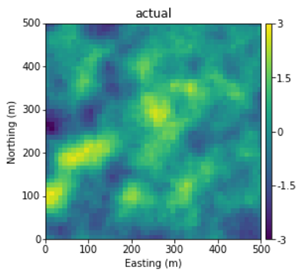
\includegraphics[width=.3\textwidth]{capitulo_3/actual.png}\label{<figure1>}}
     \subfloat[][Estimativas por SK]{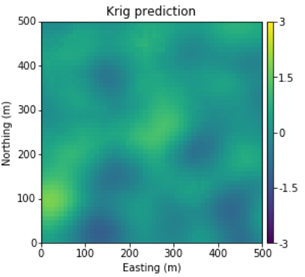
\includegraphics[width=.3\textwidth]{capitulo_3/krig.png}\label{<figure2>}}
     \subfloat[][Estimativas por ML]{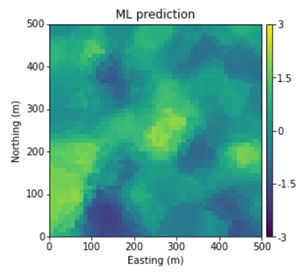
\includegraphics[width=.3\textwidth]{capitulo_3/ml.png}\label{<figure2>}}
     \legend{Fonte: \citeonline{samson_estimation_ml}}
\end{figure}

Redes neurais são baseadas em neurônios (\autoref{neuron}). Os dendritos representam o \textit{input} e os axônios representam o \textit{output}. Redes neurais são tipicamente usadas em problemas de identificação \cite{samson_intro_ml}.

\begin{figure}[!ht]
	\caption{\label{neuron}Figura esquemática de um neurônio.}
	\begin{center}
		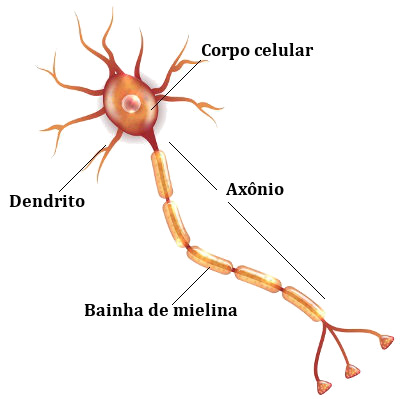
\includegraphics[width=0.3\textwidth]{capitulo_3/neuronio.jpg}
	\end{center}
	\legend{Fonte: \url{https://brasilescola.uol.com.br/o-que-e/biologia/o-que-e-neuronio.htm} acesso em: março de 2019}
\end{figure}

A \autoref{nn_ex} mostra um exemplo simples de rede neural. Os nós "x" na camada um da rede representam os \textit{inputs}, os nós "a" na camada dois e três representam as camadas escondidas, e a camada quatro é o nó de \textit{output} e representa a hipótese $H_\theta(x)$.

Redes neurais trabalham em um sistema binário de zeros e uns e por isso podem se basear nas propriedades da função sigmóide \footnote{A função sigmóide é uma função matemática de amplo uso em campos como a economia e a computação. O nome "sigmóide" vem da forma em S do seu gráfico. \cite{wiki:sigmoid}}, que tem seu valor em y entre zero e um para qualquer valor de x. Em uma rede neural uma hipótese é gerada para cada nó e é determinado se seu valor será zero ou um, o valor binário é então passado para a próxima camada. Na rede neural da \autoref{nn_ex} uma hipótese para cada nó deve ser definida, a hipótese em um nó é o peso do \textit{input} multiplicado pelo valor binário (0,1). O valor da hipótese é então imputado na função sigmóide que converte o valor para zero ou um \cite{samson_intro_ml}.

\begin{figure}[!ht]
	\caption{\label{nn_ex}Rede neural.}
	\begin{center}
		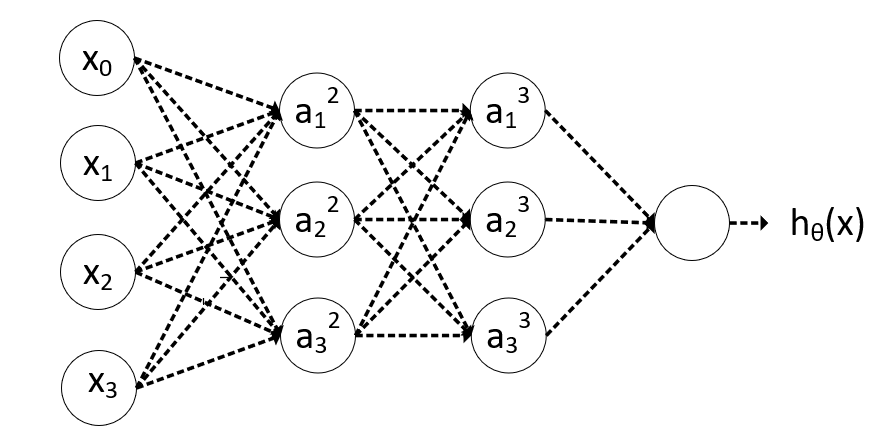
\includegraphics[width=0.7\textwidth]{capitulo_3/NN_ex.png}
	\end{center}
	\legend{Fonte: \citeonline{samson_intro_ml}}
\end{figure}

Redes neurais de bases radiais apresentam uma arquitetura semelhante às redes neurais artificiais (\autoref{nn_ex}), que consiste em uma camada de \textit{input}, camadas escondidas e uma camada de \textit{output}. A principal diferença reside no número de camadas escondidas, que nas redes neurais de bases radiais se reduz a apenas uma, além disso, redes neurais de bases radiais se baseiam em funções de bases radiais como função de ativação 

A metodologia se mostrou competente em fazer estimativas a partir de amostras esparsas sem a necessidade do cálculo e modelagem do variograma, em seu trabalho \citeonline{samson_estimation_ml}, não trinaram o parâmetro $\beta$, que controla o espalhamento da função de base radial, e sugere que isso seja feito em trabalhos futuros para otimização do método. A aplicação de redes neurais de bases radias na modelagem geológica implícita é promissora porque evita a tarefa de modelagem e cálculo do variograma, além disso, a função radial gaussiana já é utilizada com sucesso na criação dos modelos implícitos. 
%A possibilidade de inserção de anisotropia local, calculada a partir dos dados amostrais \cite{lillah2015inference}, para cada estimativa será avaliada.

\subsection{Zona de incerteza}

Um outro objetivo é desenvolver uma metodologia objetiva e direta para definição da zona de incerteza: tanto o método baseado em múltiplas categorias simultâneas (coeficiente U) \autoref{sim_direta} quanto o método da zona de incerteza calibrada (parâmetro C) \autoref{boundsim} para cada litologia de forma independente podem gerar zonas de incertezas em interseção com amostras. É necessário definir uma zona de incerteza, entre os contatos multi categóricos, que seja de fato "incerta", justa e livre de viés. Onde os contatos das múltiplas realizações devem variar. Gerar múltiplas realizações com a finalidade de avaliar a incerteza de modelos geológicos em todos os nós do \textit{grid} é desperdício de tempo e poder computacional, já que no interior dos domínios não há incerteza.

Em física a entropia é uma media do grau de desordem em um sistema. Um sistema ordenado, como um diamante, por exemplo, tem uma baixa entropia. Enquanto um sistema desordenado, como uma mistura de gases em alta temperatura, tem uma alta entropia. O conceito de entropia também surge na matemática, em teoria da probabilidade a taxa média na qual a informação é produzida por uma fonte estocástica de dados.

Desse modo, a entropia é uma medida de incerteza. A entropia da informação ou entropia de Shannon \cite{shannon1948mathematical} para um evento X com n resultados possíveis com probabilidades $(p_1, ..., p_n)$ é dada por:

\begin{equation}
    H(X)=H(p_1, ..., p_n)=-\sum^n_{i=1}p_ilog_2p_i
\end{equation}

Calcular as probabilidades de cada litologia em um determinado local é trivial, como mostrado na \autoref{heuristic} o que a torna a entropia da informação uma poderosa ferramenta tanto na definição da zona de incerteza como para de fato avaliar a incerteza do modelo geológico. Considere dois diferentes blocos onde as probabilidades de cada litologia foram calculadas e são mostradas na \autoref{entro_block}, o bloco 1 apresenta uma entropia menor que o bloco 2. Conhecimento e entropia são opostos: quando o conhecimento a respeito da mais provável litologia para um bloco é alto a entropia é baixa e vice-versa. 

\begin{figure} 
\caption{Probabilidades de para categoria em dois diferentes blocos.} \label{entro_block}
     \centering
     \subfloat[][Bloco 1]{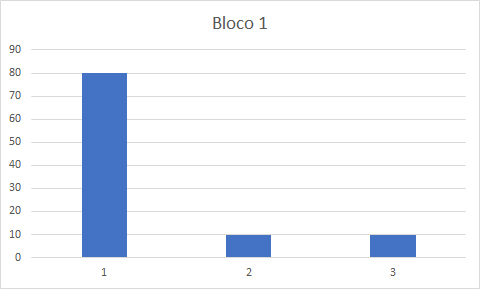
\includegraphics[width=.5\textwidth]{capitulo_3/bloco1.jpg}\label{bloco1}}
     \subfloat[][Bloco 2]{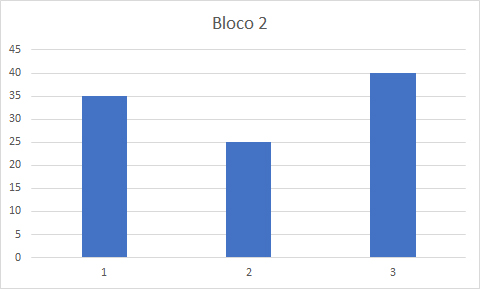
\includegraphics[width=.5\textwidth]{capitulo_3/bloco2.jpg}\label{bloco 2}}
\end{figure}

Algumas das propriedades notáveis e desejáveis da entropia são: a entropia á máxima para distribuições uniformes; é aditiva para eventos independentes; adicionar um novo evento com probabilidade zero não altera a entropia; é contínua e não negativa; a entropia para eventos como o mesmo resultado é zero; invariante à permutação.

A \autoref{entro_gamma} mostra a entropia calculada para o banco de dados em estudo a partir de probabilidades calculadas com diferentes valores de $\gamma$. A entropia, é um parâmetro semelhante ao coeficiente U (\autoref{sim_direta}), porém, a variação da entropia pode ser controlada pela magnitude das proporções calculadas pela \autoref{eq_softmax}. O parâmetro $\gamma$ deve ser calibrado para todas as litologias, levando em consideração os dados amostrais. 

\begin{figure}[t]
\caption{Entropias calculadas para diferentes valores de $\gamma$.} 
\label{entro_gamma}
\begin{center}
\subfloat[][$\gamma=20$]{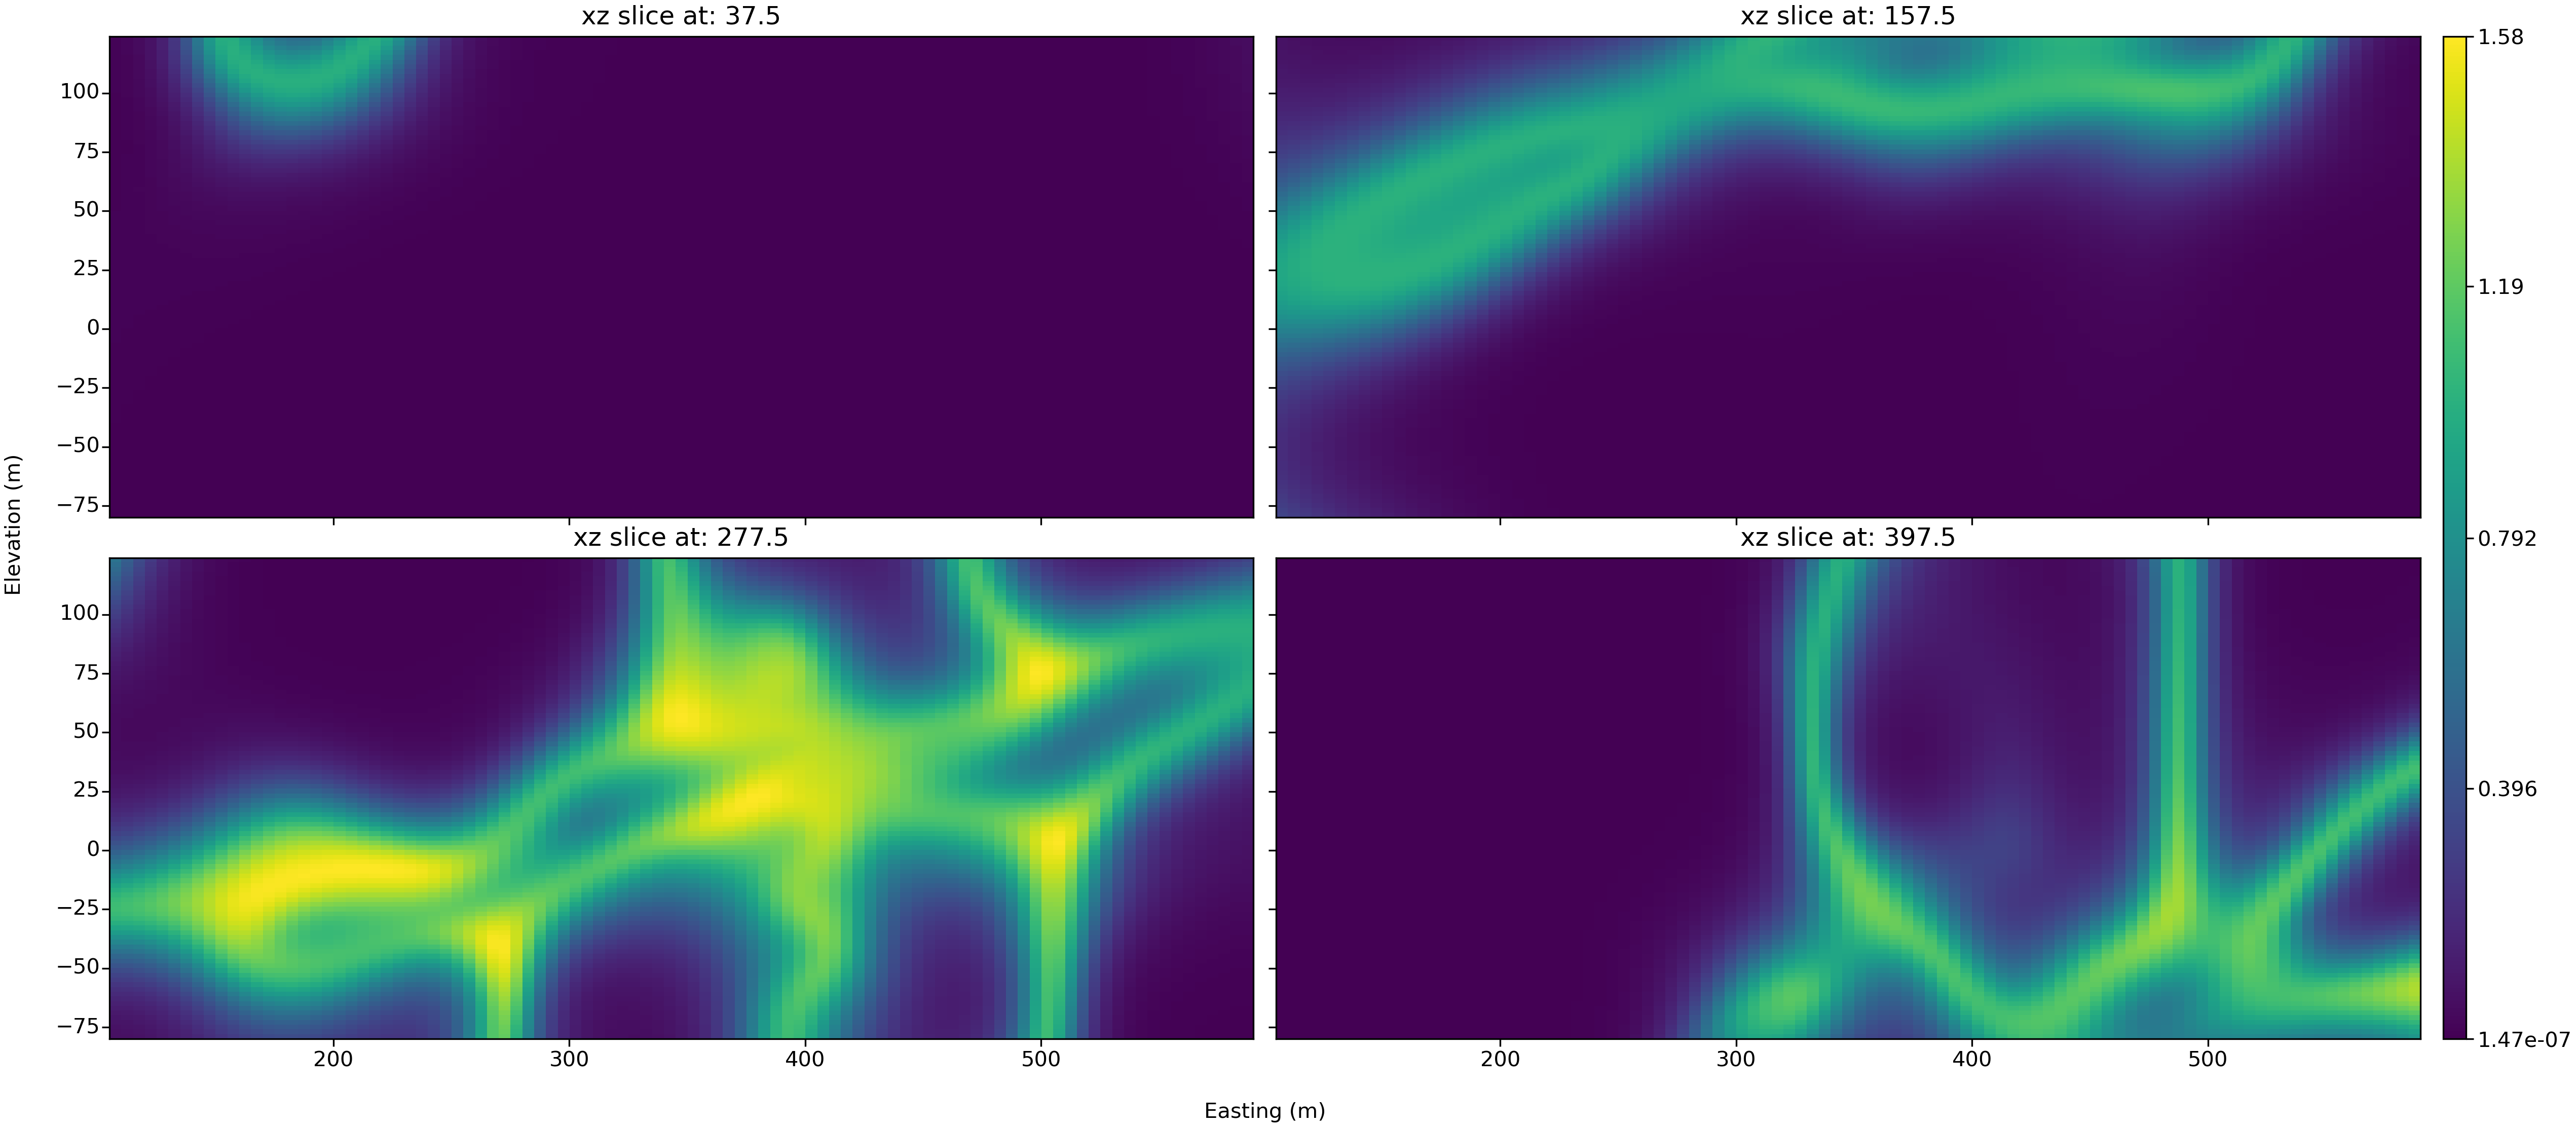
\includegraphics[width=0.8\textwidth]{capitulo_3/entropy_20.png}\label{a}}\\
\end{center}
\begin{center}
\subfloat[][$\gamma=10$]{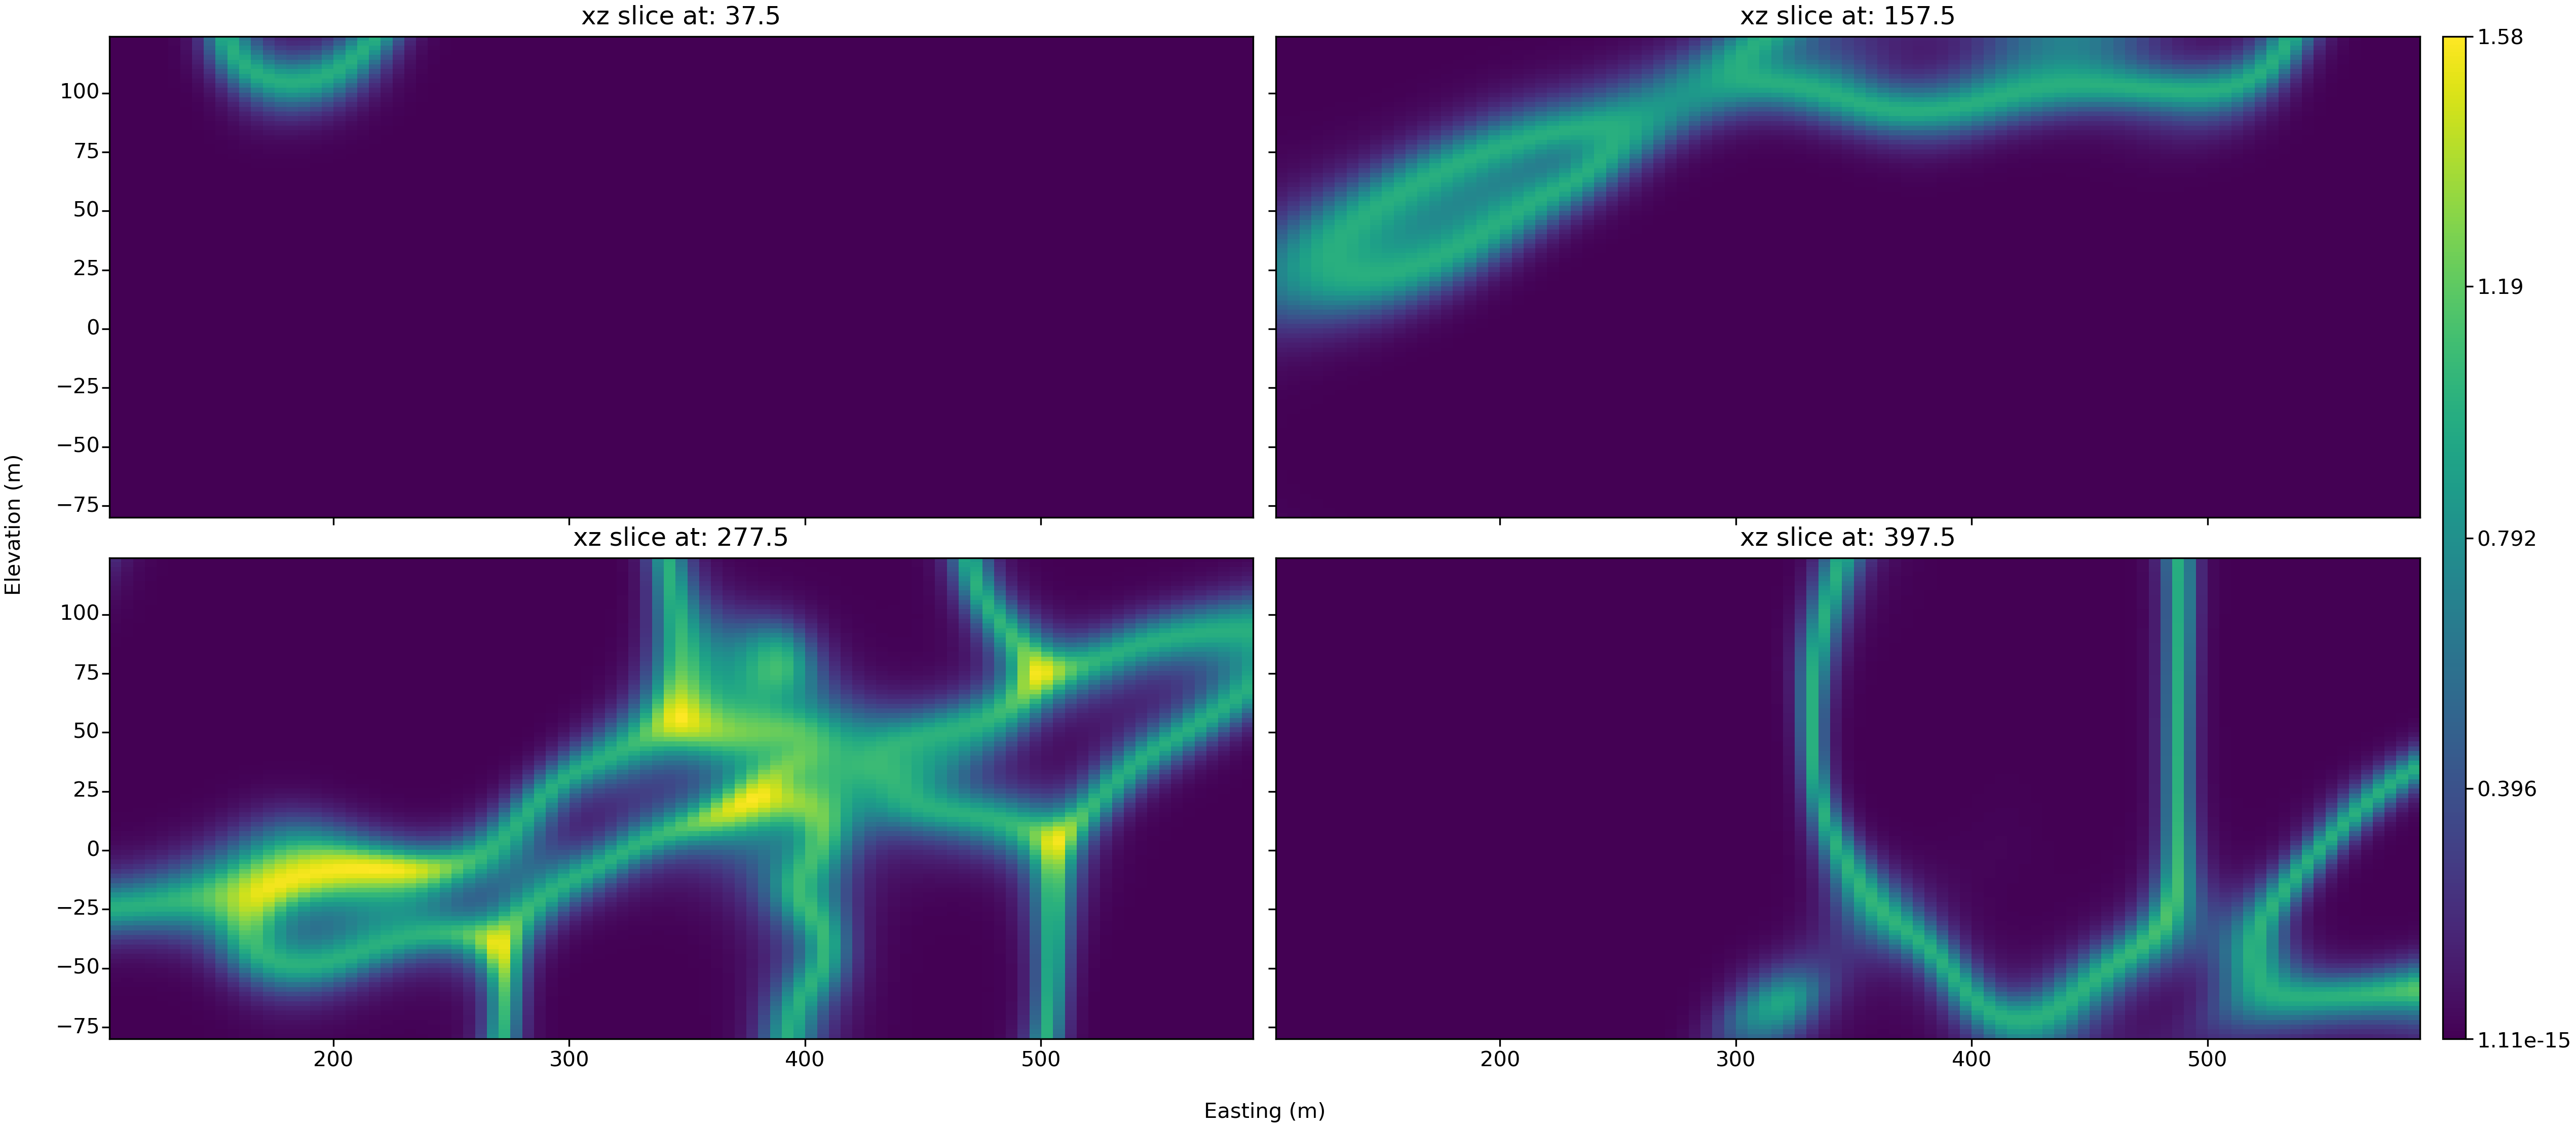
\includegraphics[width=0.8\textwidth]{capitulo_3/entropy_10.png}\label{b}}
\end{center}
\end{figure}

A probabilidade de uma dada categoria em um ponto amostral deve ser um, se a amostra pertencer à essa mesma categoria, e zero caso contrário, somando um para todas as litologias e variando de suavemente no espaço. O parâmetro $\gamma$ deveria ser calibrado de forma que na validação as duas imposições sejam atendidas, um \textit{range} de valores permissíveis para gamma pode ser definido. O $\gamma$ esolhido deve ser o que contempla a maior incerteza possível (maior valor). Dessa forma, o campo de entropia pode fornecer uma zona de incerteza de fato incerta, justa e livre de viés. A \autoref{calib_gamma} mostra a calibração do parâmetro para o banco de dados em estudo. Muitas vezes a imposição é muito restritiva e gera zonas de incerteza muito pequenas ou em alguns casos ausentes. A partir de 0.4, um valor muito pequeno para o parâmetro, já existe classificação errônea, e a partir de 110 todas as amostras são classificadas de forma errada.

\begin{figure}[!ht]
	\caption{\label{calib_gamma}Calibração do $\gamma$.}
	\begin{center}
		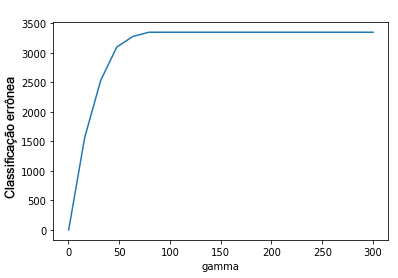
\includegraphics[width=0.7\textwidth]{capitulo_3/calib100.png}
	\end{center}
	%\legend{Fonte: \citeonline{samson_intro_ml}}
\end{figure}

Conforme o valor de $\gamma$ aumenta o número de amostras classificadas errôneamente - diferente de 0 ou diferente de 100 - aumenta, da mesma forma para todas as litologias (por isso apenas um gráfico de calibração). É preciso desenvolver uma forma de escolher o melhor valor para $\gamma$. Alguns autores recomndam escolher a maior distância estimada.

Resta então definir um \textit{cut off} no campo de entropia para sinalizar quais blocos variam e quais ficam congelados na geração dos modelos estocásticos. É preciso definir uma regra matemática, que pode ser baseada na entropia de formação do depósito mineral, depósitos de mais baixa entropia, como os de bauxita, por exemplo teriam seu \textit{cut off} definido em um valor maior do que depósitos de alta entropia, como um depósito de ouro primário.

\subsection{Avaliação de incerteza}

\subsubsection{\textit{Boundary simulation} multi categórico}

Atualmente o método de avaliação de incerteza que produz os melhores resultados é apresentado na \autoref{boundsim} esse método permite controlar o volume da zona de incerteza, e a natureza dos contatos. Nesse método o contato entre litologias varia dentro da zona de incerteza calibrada, sem a geração de ruído, além disso a natureza do contato pode ser controlada pelo variograma da simulação não condicional. Porém o método trabalha apenas com uma litologia por vez e a simulação não condicional ainda depende de um variograma. Essa tese propõe uma adaptação desse método para múltiplas categorias simultâneas. As distâncias interpoladas para as diferentes litologias serão comparadas, apenas na nova zona de incerteza, com apenas um campo simulado, dessa forma as distâncias devem ser, de alguma forma, estandardizadas, ou com n campos simulados, um para cada distância, como mostra a \autoref{comp_multi}.

\begin{figure}[!ht]
	\caption{\label{comp_multi}Comparação multi categórica.}
	\begin{center}
		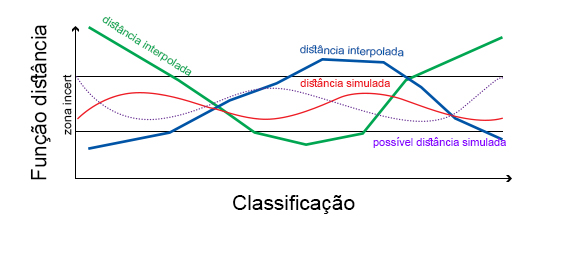
\includegraphics[width=0.8\textwidth]{capitulo_3/classificacao_multi.jpg}
	\end{center}
	%\legend{Fonte: \citeonline{samson_intro_ml}}
\end{figure}

\subsubsection{Simulação \textit{P-field}}

A ideia central desse método de simulação condicional é dissociar a tarefa de estimar distribuições de probabilidades locais para geração de múltiplas realizações equiprováveis \cite{froidevaux1993probability}. Uma premissa é de que as distribuições locais são conhecidas, o que é uma premissa razoável, já que as distribuições locais podem ser calculadas pela \autoref{eq_softmax}. As simulações condicionais são obtidas tomando valores desses CDFs locais. O valor de probabilidade usados para amostras as distribuições locais constituem o campo de probabilidades (\textit{P-field}) e são realizações de uma função aleatória caracterizada por uma distribuição uniforme e um modelo de covariância.

N realizações do campo de probabilidades podem ser geradas na zona de incerteza, para cada bloco e cada realização a litologia correspondente é tomada do CDF local a partir da probabilidade simulada naquele bloco. O variograma utilizado para geração do campo de probabilidades controla a natureza dos contatos, suave ou rugoso. É preciso definir um modelo de covariância que se adeque aos contatos de todas as litologias de forma simultânea. O uso de uma variável contínua para definir a categórica evita o surgimento de ruído nos modelos estocásticos.	

\subsubsection{Simulação plurigaussiana truncada}

Simulação gaussiana truncada (SGT) foi proposta por \citeonline{matheron1987conditional} e é uma alternativa para simular variáveis categóricas que usa uma única variável aleatória gaussiana. Realizações da variável gaussiana são tratadas como uma variável latente subjacente \cite{hier_plurigauss} e então são truncadas para gerar realizações categóricas. Todavia, o uso de apenas uma variável gaussiana faz com que a técnica seja limitada apenas a simulação de variáveis categóricas ordenadas, como ambientes sedimentares estratigráficos, por exemplo. A \autoref{trunc_gauss} mostra a variável gaussiana truncada para representar 3 diferentes categorias. A aplicação de uma regra local de truncagem na SGT gera resultados similares à simulação \textit{P-field}.

\begin{figure}[!ht]
	\caption{\label{trunc_gauss}Esquema da SGT. Note que as litologias sandstone e shale não aparecerão juntas nas realizações.}
	\begin{center}
		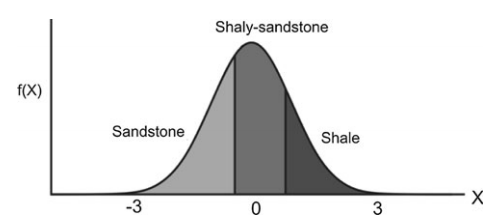
\includegraphics[width=0.5\textwidth]{capitulo_3/gauss_trunc_sketch.png}
	\end{center}
	\legend{Fonte: \citeonline{deutsch2014multidimensional}}
\end{figure}

A simulação plurigaussiana truncada (SPT), proposta por \citeonline{galli1994pros}, é uma extensão da SGT para permitir o uso de múltiplas variáveis aleatórias gaussianas (variáveis latentes), assim, permitindo a simulação de estruturas mais complexas. A SPT pode reproduzir proporções, continuidade espacial e probabilidades de transição. O poder da SPT vem do uso de múltiplas variáveis gaussianas para representar as estruturas complexas observadas nos dados. Todavia, seu uso tem sido limitado a duas funções gaussianas, $Y_1$ e $Y_2$, correlacionadas ou não, pelo fato de que a definição e interpretação de regras de truncagem é complicada em mais de duas dimensões \cite{hier_plurigauss}.

\begin{figure}[!ht]
	\caption{\label{trunc_pluri}Esquema da SPT. Note que as litologias 1 e 3 não aparecerão juntas nas realizações.}
	\begin{center}
		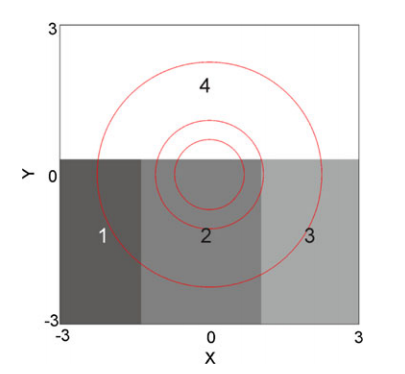
\includegraphics[width=0.5\textwidth]{capitulo_3/pluri_sketch.png}
	\end{center}
	\legend{Fonte: \citeonline{deutsch2014multidimensional}}
\end{figure}

A regra de truncagem ou regra de litologia é uma parte importante da metodologia SPT já que ela controla os contatos entre as categorias, sua transição e proporções. A definição das regras de truncagem é geralmente baseada nas probabilidades de transição observadas nos dados e nos modelos conceituais \cite{mariethoz2009truncated}. A partir dos dados, é possível calcular a probabilidade de transição de uma categoria para outra e expressá-las em forma de matriz \cite{advances_in_spt}.

\begin{figure}[!ht]
	\caption{\label{trunc_rules}Diferentes templates, para o caso de duas variáveis latentes e quatro categorias.}
	\begin{center}
		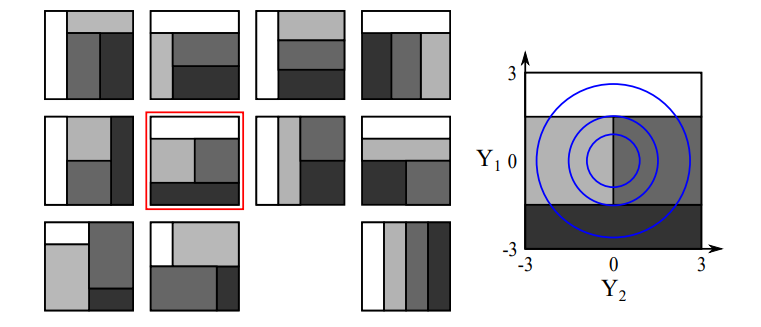
\includegraphics[width=0.5\textwidth]{capitulo_3/trunc_rules.png}
	\end{center}
	\legend{Fonte: Modificado de \citeonline{armstrong2011plurigaussian}}
\end{figure}

Diversas técnicas para definir a regra de truncagem foram propostas: \citeonline{armstrong2011plurigaussian} propões o particionamento de espaço gaussiano multivariado em paralelepípedos (ou retângulos no caso bivariado) através de limiares \autoref{trunc_rules}. Essa técnica é adequada ao caso bivariado e com poucas categorias.

\citeonline{allard2012non} introduziram o \textit{assignation diagram} que automaticamente constrói a regra de truncagem para o caso bivariado usando regressão baseada em kernel em variáveis auxiliares.

\citeonline{sadeghi_optimizing} usaram \textit{simulated annealing} para otimizar a regra de truncagem. A função objetivo é a minimização da classificação errônea entre as probabilidades de transição calculadas de realizações e das probabilidades de transição calculadas a partir dos dados.

\citeonline{deutsch2014multidimensional} usam \textit{Multidimensional scaling} (MDS) para definir regras de truncagem complexas com o foco em reproduzir as probabilidades de transição. Essa metodologia pode ser aplicada para qualquer número de variáveis gaussianas.

\citeonline{astrakova2015truncation} propuseram uma metodologia semelhante à de \citeonline{deutsch2014multidimensional} usando entropia bayesiana máxima em conjunto com \textit{simulated annealing} para otimizar a regra de truncagem bi gaussiana.

\citeonline{madani2015simulation} e \citeonline{hier_plurigauss} propuseram uma abordagem hierárquica para definir a regra de truncagem em espaços multi dimensionais.

Em muitos casos as proporções não são estacionárias, as curvas de proporção verticais, propostas por \citeonline{matheron1987conditional} mostram esse comportamento, a partir do cálculo das proporções de cada litologia a partir da profundidade. Nesses casos, a regra de truncagem não deve ser global, e deve variar localmente \cite{sadeghi_optimizing}.

Essa tese propõe a definição dinâmica da regra de truncagem bivariada para cada bloco, dentro da zona de incerteza, a partir das probabilidades calibradas e calculadas pela \autoref{eq_softmax}. A \autoref{trunc_rules_prop} mostra um desenho esquemático do método proposto.

\begin{figure}[!ht]
	\caption{\label{trunc_rules_prop}Diferentes regras de truncagem definidas para cada bloco a partir das probabilidades calibradas e calculadas.}
	\begin{center}
		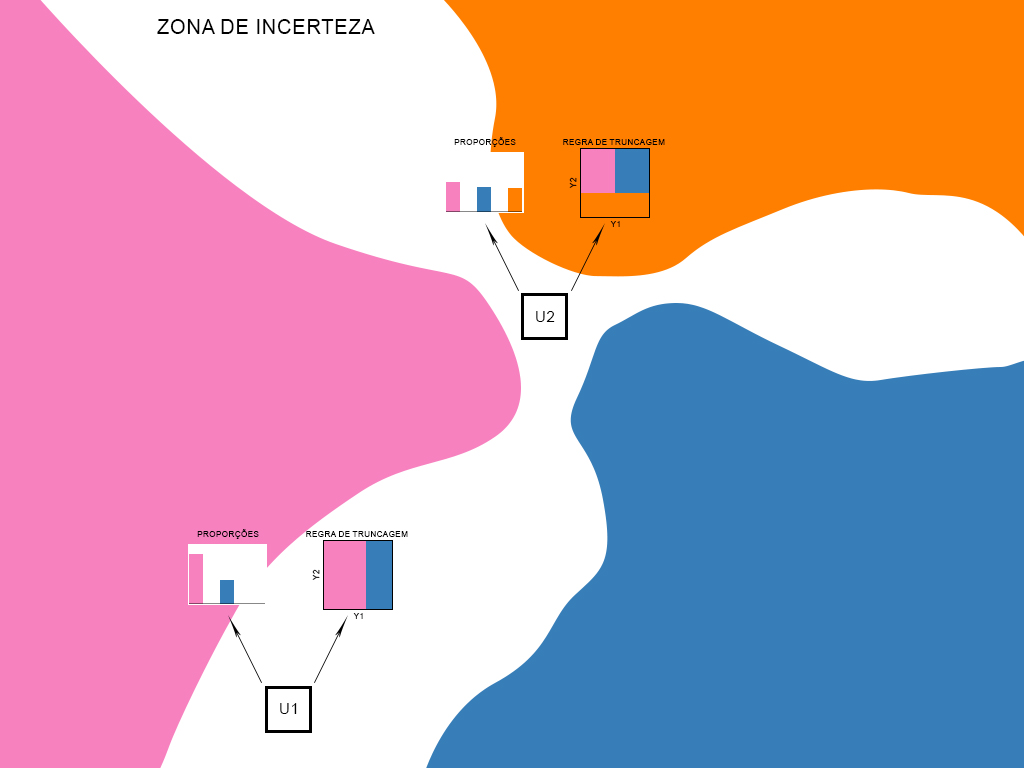
\includegraphics[width=0.6\textwidth]{capitulo_3/trunc_rules_prop.jpg}
	\end{center}
	%\legend{Fonte: Modificado de \citeonline{armstrong2011plurigaussian}}
\end{figure}

O próximo passo é simular as variáveis latentes gaussianas, cada função deve ter uma função de auto covariância. Segundo \citeonline{sadeghi_review} os variogramas devem ser modelados de forma que variável categórica original tenha a estrutura espacial correta após a truncagem. Diversas metodologias foram desenvolvidas para a definição dos variogramas. Na prática, se existem duas importantes litolgias, minério mais rico por exemplo, o variograma dessas litologias deve ser atribuídos às variáveis latentes $Y_1$ e $ Y_2$. O variograma dos indicadores deve ser invertido numericamente para corresponder ao seu variograma gaussiano \cite{journel2004evaluation} (o variograma gaussiano tem alcance e anisotropias similares  porém a forma é mais suave, é mais parabólica ou gaussiana à pequenas distâncias). Na prática o variograma dos indicadores é alterado para o modelo gaussiano \cite{pyrcz2014geostatistical}.

Na metodologia original \cite{armstrong2011plurigaussian} a simulação das variáveis latentes é condicionada valores gaussianos gerados a partir dos dados por um amostrador de Gibbs, como não existem amostras na nova zona de incerteza proposta a simulação deve ser não condicional.

O último passo é aplicar a regra de truncagem em cada bloco e para cada realização das variáveis latentes simuladas para classificar os blocos da zona de incerteza.

\subsection{Validação}

Finalmente é preciso desenvolver metodologias para validação e checagem dos modelos. A modelagem implícita tende a gerar estruturas em formatos circulares ("\textit{blobs}") ao redor das amostras, como o modelo apresentado na \autoref{blob}, ou em forma de salsicha em torno de furos de sondagem, um índice de quanto às estruturas geradas se parecem com essas estruturas indesejadas deve ser desenvolvido, bem como a checagem de locais classificados que são colocados com amostras (e devem ter sido classificados com a mesma litologia da amostra) e checagem "visual", que pode ser realizada por um algoritmo de aprendizado de máquinas.

\begin{figure}[!ht]
	\caption{\label{blob}Modelo implícito ruim, com a presença de estruturas indesejadas.}
	\begin{center}
		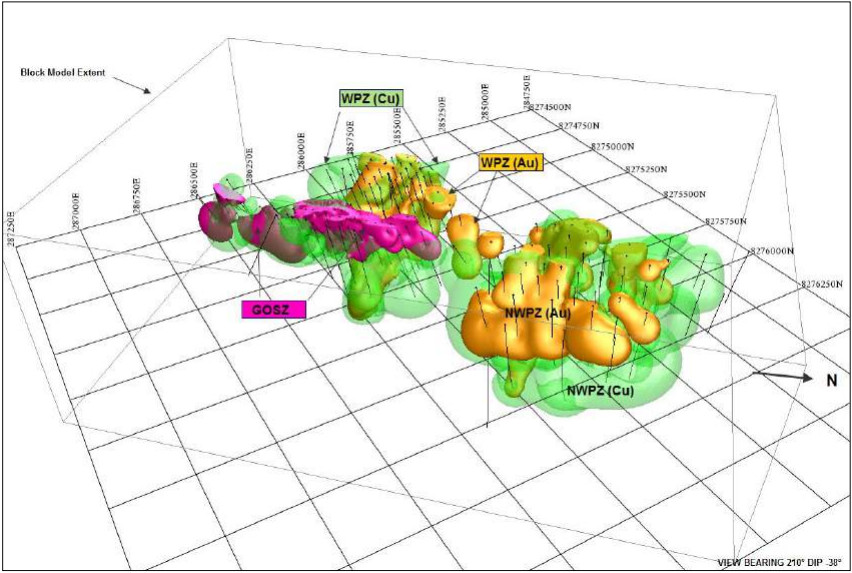
\includegraphics[width=0.7\textwidth]{capitulo_3/blob.jpg}
	\end{center}
	%\legend{Fonte: \citeonline{samson_intro_ml}}
\end{figure}

\section{Cronograma e atividades}

As atividades pretendidas para essa tese incluem: uma revisão bibliográfica da modelagem geológica implícita e todos os métodos de avaliação de incerteza disponíveis na literatura (\autoref{capitulo_2}), desenvolvimento de um pacote de modelagem geológica implícita em python que inclui ferramentas: para o calculo das distâncias, interpolação via redes neurais de bases radias, calibração das probabilidades para cada litologia, definição da zona de incerteza, e avaliação de incerteza via geração de múltiplas realizações equiprováveis do modelo geológico multi categórico e ferramentas de validação do modelo geológico.

A \autoref{cronograma} mostra o cronograma de atividades para o período da tese.

\begin{figure}[!ht]
	\caption{\label{cronograma}Cronograma de atividades.}
	\begin{center}
		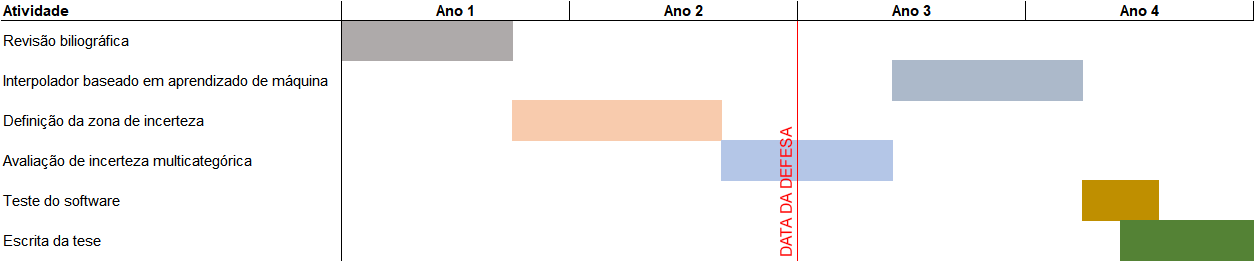
\includegraphics[width=\textwidth]{capitulo_3/cronograma_novo.png}
	\end{center}
	%\legend{Fonte: \citeonline{samson_intro_ml}}
\end{figure}